\documentclass[english]{smcca}

\usepackage{booktabs}

\title{Numerical Recovery of Forecast-Smoothness Minima: Adaptive Search, Sturm Isolation, and Temporal Matching}

\author[1]{Heriberto Espino Montelongo}
\affil[1]{Universidad de las Am\'ericas Puebla, San Andr\'es Cholula, Puebla, Mexico.}

\date{}
\setcounter{page}{1}

\newcommand{\R}{\mathbb{R}}
\newcommand{\tr}{\operatorname{tr}}

\begin{document}
\maketitle

\begin{abstract}
Selecting the smoothness of a penalized least-squares trend by
chronological forecast error yields a scalar objective over a
normalized index $S\in[0,1]$. Although the smoothing-parameter
domain $\lambda\in[0,\infty)$ is unbounded, the normalized coordinate
includes both limiting estimators and permits an explicit numerical
comparison of candidate forecast trends. The objective need not
be unimodal. We study two complementary approaches to its stationary
points: a scalable derivative-aware adaptive search with Brent
refinement and exact endpoint evaluations, and Sturm-sequence
root counting and isolation for small, exactly rationalized
finite-difference problems. The latter provides conditional
completeness on its finite polynomial instance; it does not
certify arbitrary large-window calculations. Under an earlier
frozen adaptive-search protocol, 240 relevant adversarial
optima, 2,105 synthetic dense-reference interior minima and
473 financial-data dense-reference minima were recovered;
the synthetic and financial searches used approximately
1.6--1.8\% of the corresponding dense-grid evaluation counts.
A worked six-observation Sturm example yields three positive
stationary roots, including two distinct minima. We also study
the separate numerical problem of matching minimum locations
across chronological origins. A counterexample demonstrates that
greedy nearest-neighbor matching can omit admissible links,
while existing tracking counts do not establish identity accuracy.
The paper distinguishes numerical search accuracy, conditional
root certification, and temporal matching without assuming
that they imply improved predictive performance.
\end{abstract}

\vspace{1em}

\noindent\textbf{Keywords:} penalized least squares; normalized smoothness; Sturm sequences; Brent root search; multimodal optimization; forecast validation.

\vspace{10pt}

\section{Introduction}

Quadratic penalized smoothers provide a simple way to estimate a slowly varying component from noisy observations. Their basic form goes back to Whittaker's graduation method \cite{whittaker1923graduation} and appears in time-series trend estimation as penalized least squares (PLS) \cite{guerrero2007penalized}. The smoothing parameter \(\lambda\) trades fidelity to the observed series against smoothness of the estimated trend. Small values allow the trend to follow the observations closely, whereas large values increasingly suppress penalized finite differences.

The choice of \(\lambda\) has therefore received substantial attention. Classical approaches include cross-validation (CV) and generalized cross-validation (GCV) \cite{craven1979gcv}; Cortés-Toto et al. \cite{cortes2017smoothness} implement CV, GCV, AICc, and BIC directly in the PLS framework and study the smoothness attained by each criterion. The controlled-smoothness line instead parameterizes the effect of \(\lambda\) through a trace-based smoothness index that can be interpreted in percentage terms \cite{guerrero2008smoothness,cortes2017smoothness}. Efficient numerical implementations have also been developed for Whittaker--Henderson smoothing and GCV \cite{weinert2007wh}, while Franke et al. \cite{franke2026hp} calibrate the Hodrick--Prescott smoothing parameter against known simulated trends.

Predictive selection of trend smoothness is also established. Hart \cite{hart1994tscv} introduced time-series cross-validation for kernel trend smoothing, selecting the bandwidth from one-step-ahead prediction errors based on past observations. Thus, the contribution here is not the idea of choosing smoothness by predictive performance. More generally, forecast evaluation has a well-developed temporal vocabulary: forecast origins can be fixed or rolling, models can be recalibrated as the origin advances, and training windows can be expanding or rolling \cite{tashman2000oos,bergmeir2012cv}.

Nor is the possibility of multiple minima unique to the present criterion. Biessy \cite{biessy2026wh} shows a Whittaker--Henderson example in which a GCV profile has two local minima while studying marginal-likelihood selection and numerical optimization. The problem considered here starts from these established ingredients and asks two linked numerical questions: for finite-difference PLS, how can the multiple relevant minima of a horizon-specific forecast objective be recovered efficiently and compared with the exact limiting smoothing models, and how can those minima be corresponded across neighboring chronological forecast origins when the forecasting procedure follows persistent branches through time?

The difficulty is numerical as well as statistical. The resulting forecast-validation objective is one-dimensional, but it need not have a single local minimum. A coarse grid may miss relevant minima, while a very dense grid is reliable only at a substantial evaluation cost. Searching directly in \(\lambda\in[0,\infty)\) also requires arbitrary finite bounds and devotes numerical resolution unevenly across smoothing regimes.

Our primary numerical object is the collection of stationary points and global candidates of a forecast-loss curve parameterized by $S\in[0,1]$. The bounded coordinate is a monotone rescaling of the controlled-smoothness index, so that $S=0$ and $S=1$ encode both exact limiting trends. We develop derivative-aware adaptive sampling and Brent refinement \cite{brent1971zero}, then give a distinct exact-algebra route: for small problems with rational input values, the stationary equation can be reduced to a polynomial and its positive roots counted and isolated by a Sturm sequence. The roots are mapped back to $S$ for interpretation. A further numerical question concerns matching multiple minima across nearby chronological origins.

The contribution is numerical rather than a new PLS filter or a general guarantee of predictive superiority. It comprises a fast empirical algorithm for multimodal smoothness search, a conditionally complete exact-rational solver on small inputs, and an analysis of temporal matching as a distinct assignment problem. We keep the proof scope and experiment protocols separate. The adaptive per-surface method is validated on analytic adversarial objectives, 1920 synthetic rolling forecast objectives, and 384 real financial-data objective surfaces. The exact Sturm implementation is a separate small-instance diagnostic and is not included in those performance counts. The temporal layer is demonstrated with recorded branch paths in an existing four-series experiment. Their behavior is observable but their ground-truth identities are not. We therefore also isolate the correspondence problem in a controlled benchmark design, without presenting the per-surface root-recovery success rate as a validation of temporal identity.

\section{Penalized trend estimation and forecast validation}

\subsection{Penalized least squares}

Let \(y\in\R^N\) denote an observed time series and let \(D_d\) be the matrix representing the \(d\)-th finite-difference operator, with \(1\le d<N\). Define
\[
Q=D_d^\top D_d.
\]
For a smoothing parameter \(\lambda\ge0\), the PLS trend estimate is
\begin{equation}
\widehat{\tau}_\lambda
=
\arg\min_{\tau\in\R^N}
\left\{
\|y-\tau\|_2^2
+
\lambda\|D_d\tau\|_2^2
\right\}
=
H_\lambda y,
\label{eq:pls}
\end{equation}
where
\begin{equation}
H_\lambda=(I+\lambda Q)^{-1}
\label{eq:smoother}
\end{equation}
is the smoothing matrix. This is the finite-difference PLS formulation used by Guerrero \cite{guerrero2007penalized} and belongs to the broader Whittaker--Henderson family \cite{whittaker1923graduation,weinert2007wh}.

The matrix \(Q\) has nullity \(d\). Consequently, the limit \(\lambda\to\infty\) does not eliminate the null-space component of the trend. Rather,
\[
H_\lambda
\longrightarrow
P_{\ker(D_d)},
\]
the orthogonal projector onto the null space of the difference penalty. For \(d=1\) this is the constant subspace, for \(d=2\) it is the discrete linear subspace, and higher orders give the corresponding polynomial-like limits.

\subsection{A normalized smoothness coordinate}

The controlled-smoothness literature uses the trace of the smoothing matrix to quantify attained smoothness \cite{guerrero2008smoothness,cortes2017smoothness}. For \(d\ge1\), let
\[
S_G(\lambda;N)
=
1-\frac{\tr(H_\lambda)}{N}.
\]
Because \(Q\) has \(d\) zero eigenvalues, \(S_G\) ranges from \(0\) to \(1-d/N\). For numerical search we normalize this quantity to the full unit interval:
\begin{equation}
S(\lambda)
=
\frac{N}{N-d}S_G(\lambda;N)
=
1-
\frac{1}{N-d}
\sum_{j=1}^{N-d}
\frac{1}{1+\lambda\delta_j},
\label{eq:smoothness}
\end{equation}
where \(\delta_1,\ldots,\delta_{N-d}>0\) are the positive eigenvalues of \(Q\). Thus
\[
S(0)=0,
\qquad
\lim_{\lambda\to\infty}S(\lambda)=1.
\]
The coordinate is strictly increasing because
\begin{equation}
S'(\lambda)
=
\frac{1}{N-d}
\sum_{j=1}^{N-d}
\frac{\delta_j}{(1+\lambda\delta_j)^2}
>0,
\label{eq:sprime}
\end{equation}
and it is concave:
\begin{equation}
S''(\lambda)
=
-\frac{2}{N-d}
\sum_{j=1}^{N-d}
\frac{\delta_j^2}{(1+\lambda\delta_j)^3}
<0.
\label{eq:ssecond}
\end{equation}
Equation \eqref{eq:smoothness} therefore replaces the unbounded penalty domain \([0,\infty]\) by the compact smoothness domain \([0,1]\) without changing the ordering of smoothing levels.

\subsection{Rolling forecast-validation objective}

Smoothing the historical sample and extrapolating the fitted trend are separate operations. In this paper the continuation rule is fixed to the native finite-difference continuation associated with the penalty order. Let \(G_{d,h}\) denote the linear operator that maps a fitted trend of length \(L\) to its next \(h\) continued values by imposing zero \(d\)-th finite difference beyond the forecast origin.

At forecast origin \(T\), let
\[
x_T=(y_{T-L+1},\ldots,y_T)^\top
\]
be the rolling training window and
\[
z_T=(y_{T+1},\ldots,y_{T+h})^\top
\]
the future validation block. The trend forecast is
\[
\widehat z_T(\lambda)
=
G_{d,h}H_\lambda x_T,
\]
where \(H_\lambda\) now has dimension \(L\times L\). With residual
\[
r_T(\lambda)=z_T-\widehat z_T(\lambda),
\]
the origin-specific loss is
\[
f_T(\lambda)
=
\frac{1}{h}\|r_T(\lambda)\|_2^2.
\]
For a set \(\mathcal{O}\) of rolling forecast origins, the pooled forecast-validation objective is
\begin{equation}
f_{d,L,h}(\lambda)
=
\frac{1}{|\mathcal{O}|}
\sum_{T\in\mathcal{O}}f_T(\lambda).
\label{eq:rollingloss}
\end{equation}
The trend estimator is refit at every origin using only the \(L\) observations available at that origin. The selection problem is
\begin{equation}
S^\star
\in
\arg\min_{S\in[0,1]}
F_{d,L,h}(S),
\qquad
F_{d,L,h}(S(\lambda))
=
f_{d,L,h}(\lambda).
\label{eq:selection}
\end{equation}
Thus, forecast-optimal in this paper always means optimal with respect to the rolling future-block mean squared error in \eqref{eq:rollingloss}.

\subsection{Why several forecast-CV minima can matter}

Let
\[
Q=U\operatorname{diag}(\delta_j)U^\top.
\]
In this basis the smoother attenuates penalized components through
\begin{equation}
\alpha_j(\lambda)
=
\frac{1}{1+\lambda\delta_j}.
\label{eq:spectralattenuation}
\end{equation}
The attenuation is component-specific: as \(\lambda\) changes, different
penalized directions disappear at different rates. Consequently, the fitted
endpoint level, slope, and higher-order finite differences can change
substantially across smoothing levels. The continuation operator then maps
those endpoint features into future values.

This provides a mechanism by which several local minima can arise. A rougher
trend can preserve recent movement and extrapolate a stronger local slope or
curvature, while a smoother trend can suppress that movement and extrapolate a
more stable low-frequency path. Their forecast errors can cross across rolling
origins, so the average objective in \eqref{eq:rollingloss} need not be unimodal.
The existence of multiple minima is therefore a property to diagnose rather
than an assumption imposed on every series.

\subsection{Analytic derivatives}

The derivative of the smoothing matrix follows from differentiating a matrix inverse:
\[
H_\lambda'
=
-H_\lambda QH_\lambda,
\qquad
H_\lambda''
=
2H_\lambda QH_\lambda QH_\lambda.
\]
Define
\[
a_T(\lambda)
=
G_{d,h}H_\lambda QH_\lambda x_T,
\]
and
\[
b_T(\lambda)
=
G_{d,h}H_\lambda QH_\lambda QH_\lambda x_T.
\]
Then
\begin{align}
f_T'(\lambda)
&=
\frac{2}{h}r_T(\lambda)^\top a_T(\lambda),
\label{eq:firstforecast}
\\
f_T''(\lambda)
&=
\frac{2}{h}
\left[
\|a_T(\lambda)\|_2^2
-
2r_T(\lambda)^\top b_T(\lambda)
\right].
\label{eq:secondforecast}
\end{align}
The derivatives of the pooled objective are obtained by averaging \eqref{eq:firstforecast}--\eqref{eq:secondforecast} over forecast origins.

The monotone change of coordinate preserves the interior stationary points:
\begin{equation}
F'(S)
=
\frac{f'(\lambda)}{S'(\lambda)}.
\label{eq:chainfirst}
\end{equation}
Moreover,
\begin{equation}
F''(S)
=
\frac{f''(\lambda)}{[S'(\lambda)]^2}
-
\frac{f'(\lambda)S''(\lambda)}{[S'(\lambda)]^3}.
\label{eq:chainsecond}
\end{equation}
At a stationary point \(f'(\lambda^\star)=0\), the second term vanishes and the sign of the curvature is preserved. We can therefore search in the compact \(S\)-domain while evaluating analytic derivatives through \(\lambda\).

\section{Adaptive search on the smoothness domain}

The numerical target is the set of relevant local minima of \(F(S)\), together with the exact smoothness-domain endpoints. The algorithm does not assume that \(F\) is unimodal.

The frozen procedure begins with nine uniformly spaced points over the interior search interval and augments the first and last coarse cells with six levels of deterministic dyadic refinement. The additional endpoint resolution is important because the map \(S(\lambda)\) compactifies an unbounded \(\lambda\)-domain; distinct features at large \(\lambda\) can therefore become compressed close to \(S=1\).

Each sampled point provides the objective, gradient, and curvature in the smoothness coordinate through \eqref{eq:chainfirst}--\eqref{eq:chainsecond}. An interval is subdivided when the sampled derivatives indicate unresolved structure: a turning gradient, a change in curvature sign, a midpoint derivative that is small relative to the endpoint derivatives, or a pattern consistent with more than one sign change inside the interval. Subdivision stops at maximum depth eight or interval width \(10^{-3}\). The frozen derivative and curvature tolerances are \(10^{-8}\), the relative near-zero threshold is \(0.2\), and the interior upper boundary is \(1-10^{-6}\).

After adaptive sampling, every derivative sign change is bracketed and refined with Brent's method \cite{brent1971zero} to a root tolerance of \(10^{-10}\). Stationary points are classified by the sign of \(F''(S)\). The global selected value is the best among all detected local minima and the two exact endpoint candidates:
\[
S=0\Longleftrightarrow\lambda=0,
\qquad
S=1\Longleftrightarrow\lambda=\infty.
\]
The \(S=1\) objective is evaluated through the exact null-space limit rather than by replacing one with a value such as \(0.999999\).

When several nearby minima are useful for downstream inspection, a within-surface post-processing spacing radius may be applied after discovery. Candidates are ordered by objective value and worse minima inside that radius are suppressed. This quantity is denoted \(\varepsilon_{\mathrm{space}}\) here to distinguish it from the temporal tracking radius introduced below. Because spacing occurs after root discovery and ranking, it does not change the selected best minimum. The frozen numerical benchmarks below therefore assess the search before this optional summarization step.

No finite adaptive sampler can certify recovery of every stationary point of an arbitrary smooth scalar function. The empirical validation is consequently designed around missed local minima, selected-smoothness error, positive objective regret, and evaluation cost rather than a universal root-recovery claim.

\subsection{Exact Sturm root isolation for small rational instances}
\label{sec:sturm}

The adaptive search above is numerical and cannot prove that every
stationary point of a general smooth objective has been found. For
the finite-difference PLS model with rational observations and a
fixed finite forecast operator, an exact alternative exists in
small dimensions. Because
\begin{equation}
\label{eq:sturm_rational}
H_{\lambda}=(I+\lambda D_d^\top D_d)^{-1},
\qquad
f(\lambda)=\frac{P(\lambda)}{R(\lambda)},
\end{equation}
with polynomial numerator and denominator over the rational
numbers, differentiation yields another rational function
\begin{equation}
\label{eq:sturm_derivative}
f'(\lambda)=\frac{N(\lambda)}{D(\lambda)}.
\end{equation}
For $\lambda\ge0$, the matrix $I+\lambda D_d^\top D_d$
is positive definite, hence the reduced rational
denominator has no poles on the search half-line. Positive
interior stationary points are therefore exactly the positive
roots of $N$. Let $N_{\mathrm{sf}}$ denote the square-free part of $N$.
Its Sturm chain \cite{basu2006algorithms} is
\begin{equation}
\label{eq:sturm_chain}
p_0=N_{\mathrm{sf}},\qquad p_1=N_{\mathrm{sf}}',\qquad
p_{k+1}=-\operatorname{rem}(p_{k-1},p_k).
\end{equation}
The variation count of this exact polynomial sequence gives
the number of distinct stationary roots. In particular, for roots in $(0,\infty)$,
\begin{equation}
\label{eq:sturm_count}
n_{+}=V(0^+)-V(+\infty).
\end{equation}
Zero entries in a sign list are omitted; at positive infinity
each polynomial has the sign of its leading coefficient.
Repeated roots require square-free handling for the Sturm
count and must be preserved with their multiplicities in the
reported isolated-root intervals. A stationary point of even
multiplicity may have no derivative sign change and can be
missed by ordinary Brent bracketing alone.

The implementation \texttt{sturm\_forecast\_smoothness} constructs
the exact rational forecast MSE for one or several pooled
historical origins, isolates every positive stationary root
with rational intervals, classifies its local behavior, and
includes both exact limiting endpoint losses in the global
comparison. This is a symbolic calculation in $\lambda$
\emph{only because} that coordinate makes the rational
polynomial representation algebraically accessible.
The reported and optimized \emph{statistical} smoothness
coordinate remains
\begin{equation}
\label{eq:sturm_map_to_s}
S_j=S(\lambda_j)\in(0,1),
\qquad
S(0)=0,\quad S(\infty)=1.
\end{equation}
Thus the exact algebraic auxiliary variable should not be
confused with the search/reporting parameter $S$.

The exact-root count certifies completeness for the
\emph{finite rationalized objective} built from the supplied
decimal inputs. It does not certify arbitrary floating-point
data-generating mechanisms, interval arithmetic of the
reported approximate root coordinates, or the large-window
experiments. Symbolic inversion and high-degree polynomial
remainders scale poorly; the implementation consequently
rejects windows larger than eight observations by default.
It is an opt-in diagnostic and an exact small-window
alternative, not a silent replacement for the scalable
adaptive solver. Run it with
\texttt{python experiments/numerical\_smoothness\_selection/run\_sturm\_minicheck.py}
after installing the optional \texttt{symbolic} dependencies.

\subsection{Temporal correspondence of local minima}
\label{sec:tracking}

Let
\[
\mathcal M_t=\{S_{1,t},\ldots,S_{K_t,t}\}
\]
be the local minima recovered at chronological forecast origin $t$.
Given a set of active branches at $t-1$ and the current minimum set
$\mathcal M_t$, a matching defines an injective partial map from previous
branches to current candidates. A pair is admissible only if
\begin{equation}
\label{eq:track_epsilon}
|S_{j,t-1}-S_{k,t}|\le\varepsilon_{\mathrm{track}}.
\end{equation}
The partial-map formulation permits unmatched previous branches and
unmatched current minima. The latter may represent newly appearing
minima, but automatic birth initialization is a separate policy rather than
a consequence of pairwise matching.

The temporal radius $\varepsilon_{\mathrm{track}}$ is distinct from the
within-surface representative-spacing radius $\varepsilon_{\mathrm{space}}$:
the first controls the links between origins; the second may summarize
candidates already recovered on a single surface. Neither radius
constitutes a statistical confidence threshold.

The implemented baseline constructs all admissible previous--current
pairs, sorts them by increasing absolute smoothness distance, and
accepts each pair provided neither endpoint has already been matched.
This greedy one-to-one algorithm is deterministic under its tie-breaking,
but is not necessarily optimal even for a pair of neighboring origins.
For example, suppose two previous branches lie at $0.40$ and $0.48$,
and the current candidates are $0.34$ and $0.43$, with
$\varepsilon_{\mathrm{track}}=0.10$. The shortest pair links $0.40$ to
$0.43$ at cost $0.03$, leaving $0.48$ unmatched because its distance to
$0.34$ exceeds the radius. Yet two admissible pairs exist: $0.40$
to $0.34$ at distance $0.06$ and $0.48$ to $0.43$ at distance $0.05$.

This suggests a distinct pairwise assignment criterion. For admissible
links $E_t$, find a partial one-to-one matching $A_t\subseteq E_t$
lexicographically minimizing
\begin{equation}
\label{eq:assignment}
\left(
-|A_t|,
\sum_{(j,k)\in A_t}|S_{j,t-1}-S_{k,t}|
\right).
\end{equation}
The first component maximizes the number of continued branches;
conditional on that, the second minimizes total displacement. This
is a pairwise criterion, not a joint minimum-cost path across all times.
It also does not establish correct physical branch identity when minima
cross or become observationally indistinguishable: the nearest-position
assignment can exchange their underlying labels.

The existing rolling experiment initializes up to five branches at its
first origin and attempts to continue them in later origins. It records
unmatched states but does not automatically create new branches from
unassigned current minima. A separate controlled diagnostic compares
the greedy matcher with the exact pairwise objective
\eqref{eq:assignment}; true identities are known only in that synthetic
diagnostic. This distinction prevents observed temporal smoothness
paths from being mistaken for certified correspondence.

\section{Experimental design}

\subsection{Adversarial analytic objectives}

Nine deterministic polynomial objectives were constructed directly in the \(S\)-domain with known stationary structure. They include minima near both endpoints, two close minima, two close upper-tail minima, a flat quartic minimum, five separated minima, exact boundary optima, and a stationary inflection that is not a local minimum. Each shape was transformed through the \(S\leftrightarrow\lambda\) map for
\[
N\in\{63,126,252,504\},
\qquad
d\in\{1,2,3,4\},
\]
giving 144 method configurations. The frozen adaptive search was compared with a 20\,001-point dense \(S\)-grid and a 257-point uniform search in \(\log\lambda\), with derivative roots refined after bracketing.

\subsection{Synthetic forecast-validation surfaces}

Synthetic observations follow a local-linear latent trend with AR(1) observation noise. The latent slope evolves as a random walk and the observed series is the latent trend plus stationary AR(1) noise. Three regimes were used: baseline \((\sigma_{\Delta\text{slope}}=0.01,\sigma_\eta=0.5,\phi=0.3)\), persistent noise \((0.01,0.5,0.8)\), and a rougher latent trend \((0.03,0.5,0.3)\).

Each series has 800 observations. The paper-scale benchmark crosses ten random seeds with
\[
d\in\{1,2,3,4\},\quad
L\in\{63,126,252,504\},\quad
h\in\{1,5,20,60\},
\]
for a total of 1920 forecast-validation surfaces. Rolling windows advance in steps of five observations and the last 30 valid origins are scored. Each adaptive result is compared with a 5001-point dense reference grid on \([0,1]\).

\subsection{Real-data geometry stress test}

The final external check uses six versioned daily closing-price series: SPY, QQQ, AAPL, XOM, BTC--USD, and ETH--USD. The final 2000 positive observations of each tracked snapshot are transformed to natural logarithms. The same four orders, four window lengths, and four horizons used in the synthetic benchmark produce
\[
6\times4\times4\times4=384
\]
real-data objective surfaces. These experiments test numerical geometry only; they are not a comparison of financial forecasting models and are not interpreted as evidence of return or price predictability.

\subsection{Applied development/test case studies}

To interpret the numerical minima, a separate applied experiment uses four
pre-specified tracked series: quarterly U.S. real GDP (GDPC1), SPY, AAPL, and
BTC--USD. The final eight quarters of GDP and the final 60 observations of each
daily market series are reserved before any configuration search. All positive
levels are modeled on the natural-log scale.

Within the development region, the pre-specified \((d,L,h)\) grid is scanned
using the frozen search. Candidate minima are summarized with the already
frozen spacing radius \(\varepsilon=0.10\), retaining at most three
representatives ranked by rolling forecast-CV error. Among configurations with
at least two representatives, the displayed case maximizes the smoothness
separation between its two lowest-CV candidates, with lexicographic
\((d,L,h)\) tie breaking. This rule uses development data only.

After the candidate set is frozen, each candidate is refit at the final
development origin and scored on the first \(h\) observations of the untouched
test block. A validation--test rank reversal is recorded when the lowest-CV
candidate is not the lowest-test-error candidate among this already frozen set.
The test ranking is retrospective diagnostic information; it is never fed back
into candidate or configuration selection.

\subsection{Temporal tracking demonstration and controlled design}
\label{sec:tracking_design}

A chronological tracking demonstration was carried out on the versioned
GDPC1, SPY, AAPL, and BTC--USD series. For each difference order, the
window length was chosen from historical Validation-1 loss before tracking.
The maximum number of initialized minima was five, with
$\varepsilon_{\mathrm{space}}=0.02$ and
$\varepsilon_{\mathrm{track}}=0.10$. The maximum number of historical
paired validation origins was 24 for GDP and 30 for the daily series.
The numerical output records branch identifiers, matched and missing
origins, smoothness values, continuation distances, and current
candidate counts. Validation-2 and true-test forecast scores are
recorded in the underlying rolling-origin demonstration and are
not treated as tests of numerical branch identity.

A separate controlled benchmark is specified in
\texttt{CP05\_TRACKING\_CORRESPONDENCE.md}. It feeds known labeled
minima to the existing greedy algorithm and an exact pairwise
maximum-cardinality/minimum-distance comparator. The simulated
mechanisms include separated branches, gradual drift, a near-merger,
crossing paths, and branch birth/death. The continuation radii are
$\{0.03,0.06,0.10,0.15\}$ over 42 origins. Comparisons use 100 seeds in
the paper preset. At each adjacent pair, previous candidates are reset
to their known true labels to isolate one-step correspondence errors.
The benchmark therefore does not claim to validate full multi-time
tracking under accumulated labeling mistakes. Its numerical results
will be added only after the independent preset is run and committed.

\subsection{Frozen protocol and sensitivity}

The primary search specification was frozen after a pre-paper quick benchmark and before the 1920-surface confirmatory run. A separate one-factor-at-a-time sensitivity analysis then varied the initial grid size, maximum depth, endpoint-refinement levels, minimum interval width, and near-zero derivative threshold while leaving all other settings fixed.

A dense-grid local minimum is counted as recovered when an adaptive local minimum lies within two dense-grid cells. Positive objective regret is
\[
\max\{F(\widehat S)-F(S_{\mathrm{ref}}),0\},
\]
with values below \(10^{-12}\) treated as numerical roundoff. Because the adaptive root refinement is continuous while the reference is discrete, a negative raw regret can occur when the adaptive method locates a lower point between two grid nodes.

\section{Results}

Table \ref{tab:benchmark} summarizes the three frozen benchmark families. The adaptive search recovered every relevant known adversarial minimum or boundary optimum (240/240), every dense-reference interior minimum in the synthetic benchmark (2105/2105), and every dense-reference interior minimum in the financial stress test (473/473). No benchmark case had positive objective regret beyond the numerical threshold.

\begin{table}[H]
\centering
\caption{Frozen benchmark summary. Evaluation fraction is the mean adaptive evaluation count divided by the corresponding dense-grid count.}
\label{tab:benchmark}
\resizebox{\textwidth}{!}{\begin{tabular}{lrrrrrrr}
\toprule
Benchmark & Surfaces & Minima recovered & Positive-regret cases & Mean evals. & Dense evals. & Eval. fraction & Max $|\Delta S^\star|$ \\
\midrule
Adversarial & 144 & 240/240 & 0 & 75.2 & 20001 & 0.38\% & $9.06\times 10^{-5}$ \\
Synthetic & 1920 & 2105/2105 & 0 & 78.4 & 5001 & 1.57\% & $1.02\times 10^{-4}$ \\
Financial & 384 & 473/473 & 0 & 91.9 & 5001 & 1.84\% & $9.98\times 10^{-5}$ \\
\bottomrule
\end{tabular}
}
\end{table}

On the synthetic forecast surfaces, the adaptive search required 78.35 evaluations on average versus 5001 for the dense reference, or 1.57\% of the dense evaluation count. The maximum difference between the selected adaptive smoothness and the dense-grid choice was \(1.02\times10^{-4}\), approximately one half of a dense-grid cell. Total measured runtime was 27.29 seconds for the adaptive search and 1497.85 seconds for the dense reference on the benchmark machine. The wall-clock ratio is implementation- and hardware-dependent, so the evaluation-count comparison is the more portable computational result.

The financial stress test showed similar behavior: 91.89 adaptive evaluations on average versus 5001 dense evaluations, an evaluation fraction of 1.84\%, with maximum selected-\(S\) discrepancy \(9.98\times10^{-5}\). Measured total runtime was 6.52 seconds for the adaptive search and 292.97 seconds for the dense reference.

\begin{figure}[H]
\centering
\includegraphics[width=0.93\textwidth]{evaluation_efficiency.pdf}
\caption{Mean evaluation counts across the frozen benchmarks. The vertical axis is logarithmic. One adaptive evaluation returns the objective and its first two derivatives, whereas a dense-grid evaluation requires only the objective; measured wall-clock times are therefore reported separately in the text.}
\label{fig:efficiency}
\end{figure}

Figure \ref{fig:agreement} compares the smoothness selected by the adaptive search with the dense reference for all synthetic and financial surfaces. The points are concentrated on the identity line throughout the unit interval, including cases where the optimum lies near a smoothness-domain endpoint.

\begin{figure}[H]
\centering
\includegraphics[width=0.72\textwidth]{optimum_agreement.pdf}
\caption{Agreement between adaptive and dense-reference selected smoothness for the 1920 synthetic and 384 financial objective surfaces.}
\label{fig:agreement}
\end{figure}

Exact endpoint handling was not merely formal. In the synthetic benchmark, the selected optimum was interior in 1574 surfaces, \(S=0\) in 312, and \(S=1\) in 34. In the financial stress test, the corresponding counts were 321, 53, and 10. Replacing \(S=1\) by a large but finite \(\lambda\) would therefore alter a non-negligible part of the benchmark protocol.

The adversarial benchmark also separates the proposed search from a simple alternative parametrization. The uniform \(\log\lambda\) stationary search detected 226 of 240 relevant known minima or boundary optima and required 273.44 evaluations on average. Its misses were concentrated in the deliberately close-minimum constructions. The adaptive \(S\)-search detected all 240 with 75.24 mean evaluations. The stationary-inflection target was not detected by the adaptive method or by the dense local-minimum detector, but it is not an optimization candidate and is outside the primary claim.

The sensitivity study explains which parts of the frozen specification matter. Table \ref{tab:sensitivity} reports the one-factor variants. Initial grid sizes from 5 to 13, maximum depths from 4 to 10, tested minimum interval widths, and endpoint refinement of at least two levels all recovered every reference minimum in the 216-surface sensitivity panel. In contrast, removing endpoint refinement missed five minima, produced positive regret in three cases, and increased the maximum selected-\(S\) error to \(1.85\times10^{-2}\). Reducing the near-zero derivative ratio from 0.2 to 0.1 missed one secondary local minimum, although it did not change the selected global optimum.

\begin{table}[H]
\centering
\caption{One-factor-at-a-time sensitivity around the frozen primary specification. The sensitivity study is diagnostic; it was not used to retune the confirmatory algorithm after the final benchmark.}
\label{tab:sensitivity}
\resizebox{0.90\textwidth}{!}{\begin{tabular}{lrrrr}
\toprule
Specification & Missed minima & Positive-regret cases & Mean evals. & Max $|\Delta S^\star|$ \\
\midrule
Primary & 0 & 0 & 82.8 & $9.92\times 10^{-5}$ \\
initial\_grid\_size=5 & 0 & 0 & 75.4 & $9.92\times 10^{-5}$ \\
initial\_grid\_size=7 & 0 & 0 & 83.0 & $9.92\times 10^{-5}$ \\
initial\_grid\_size=13 & 0 & 0 & 93.8 & $9.92\times 10^{-5}$ \\
max\_depth=4 & 0 & 0 & 71.5 & $9.92\times 10^{-5}$ \\
max\_depth=6 & 0 & 0 & 80.0 & $9.92\times 10^{-5}$ \\
max\_depth=10 & 0 & 0 & 82.8 & $9.92\times 10^{-5}$ \\
endpoint\_refinement\_levels=0 & 5 & 3 & 64.0 & $1.85\times 10^{-2}$ \\
endpoint\_refinement\_levels=2 & 0 & 0 & 70.2 & $9.92\times 10^{-5}$ \\
endpoint\_refinement\_levels=4 & 0 & 0 & 75.5 & $9.92\times 10^{-5}$ \\
endpoint\_refinement\_levels=8 & 0 & 0 & 90.8 & $9.92\times 10^{-5}$ \\
min\_interval=0.0005 & 0 & 0 & 88.8 & $9.92\times 10^{-5}$ \\
min\_interval=0.002 & 0 & 0 & 76.8 & $9.92\times 10^{-5}$ \\
min\_interval=0.005 & 0 & 0 & 70.8 & $9.92\times 10^{-5}$ \\
near\_zero\_ratio=0.1 & 1 & 0 & 82.1 & $9.92\times 10^{-5}$ \\
near\_zero\_ratio=0.5 & 0 & 0 & 92.7 & $9.92\times 10^{-5}$ \\
\bottomrule
\end{tabular}
}
\end{table}

\begin{figure}[H]
\centering
\includegraphics[width=0.82\textwidth]{sensitivity_tradeoff.pdf}
\caption{Evaluation cost and missed-reference-minimum count in the one-factor sensitivity study. The main observed failure mode is the removal of endpoint-aware refinement.}
\label{fig:sensitivity}
\end{figure}

The optional \(\varepsilon\)-spacing rule affects only how multiple detected minima are summarized. With \(\varepsilon=0.10\), 359 nearby candidates were suppressed across 330 synthetic surfaces, while the best detected minimum in each surface was preserved by construction.

\subsection{Applied interpretation of multiple minima}

The applied scan confirms that multimodality is not universal. None of the 64
pre-specified GDP configurations produced two \(\varepsilon\)-separated
representative minima. In contrast, this occurred in 7/64 SPY configurations,
10/64 AAPL configurations, and 9/64 BTC--USD configurations; three BTC
configurations produced three representatives. GDP therefore provides a useful
unimodal contrast to the market examples.

The selected SPY case used \(d=1\), \(L=126\), and \(h=60\). Rolling CV ranked
an interior minimum at \(S=0.95639\) first, with MSE \(0.00177070\), and the
exact lower endpoint \(S=0\) second, with MSE \(0.00195813\). Thus the endpoint
candidate had about 10.6\% larger validation error. After freezing these two
candidates, their test MSE values were \(0.00093985\) and \(0.00066164\),
respectively. The validation ordering therefore reversed: the second-ranked
validation candidate had about 29.6\% lower test MSE on the later block.

The AAPL case produced two widely separated minima,
\(S=0.62901\) and \(S=0.99733\), but the second had much larger validation and
test error. The selected BTC--USD case produced three representatives at
\(S=0.84463\), \(0.02908\), and \(0.99786\). Its second candidate was only
about 13.9\% worse than the winner in rolling CV, yet its test MSE was about
14.7 times larger. These examples show that separated minima can range from
competitive alternatives to clearly inferior local optima.

\begin{figure}[p]
\centering
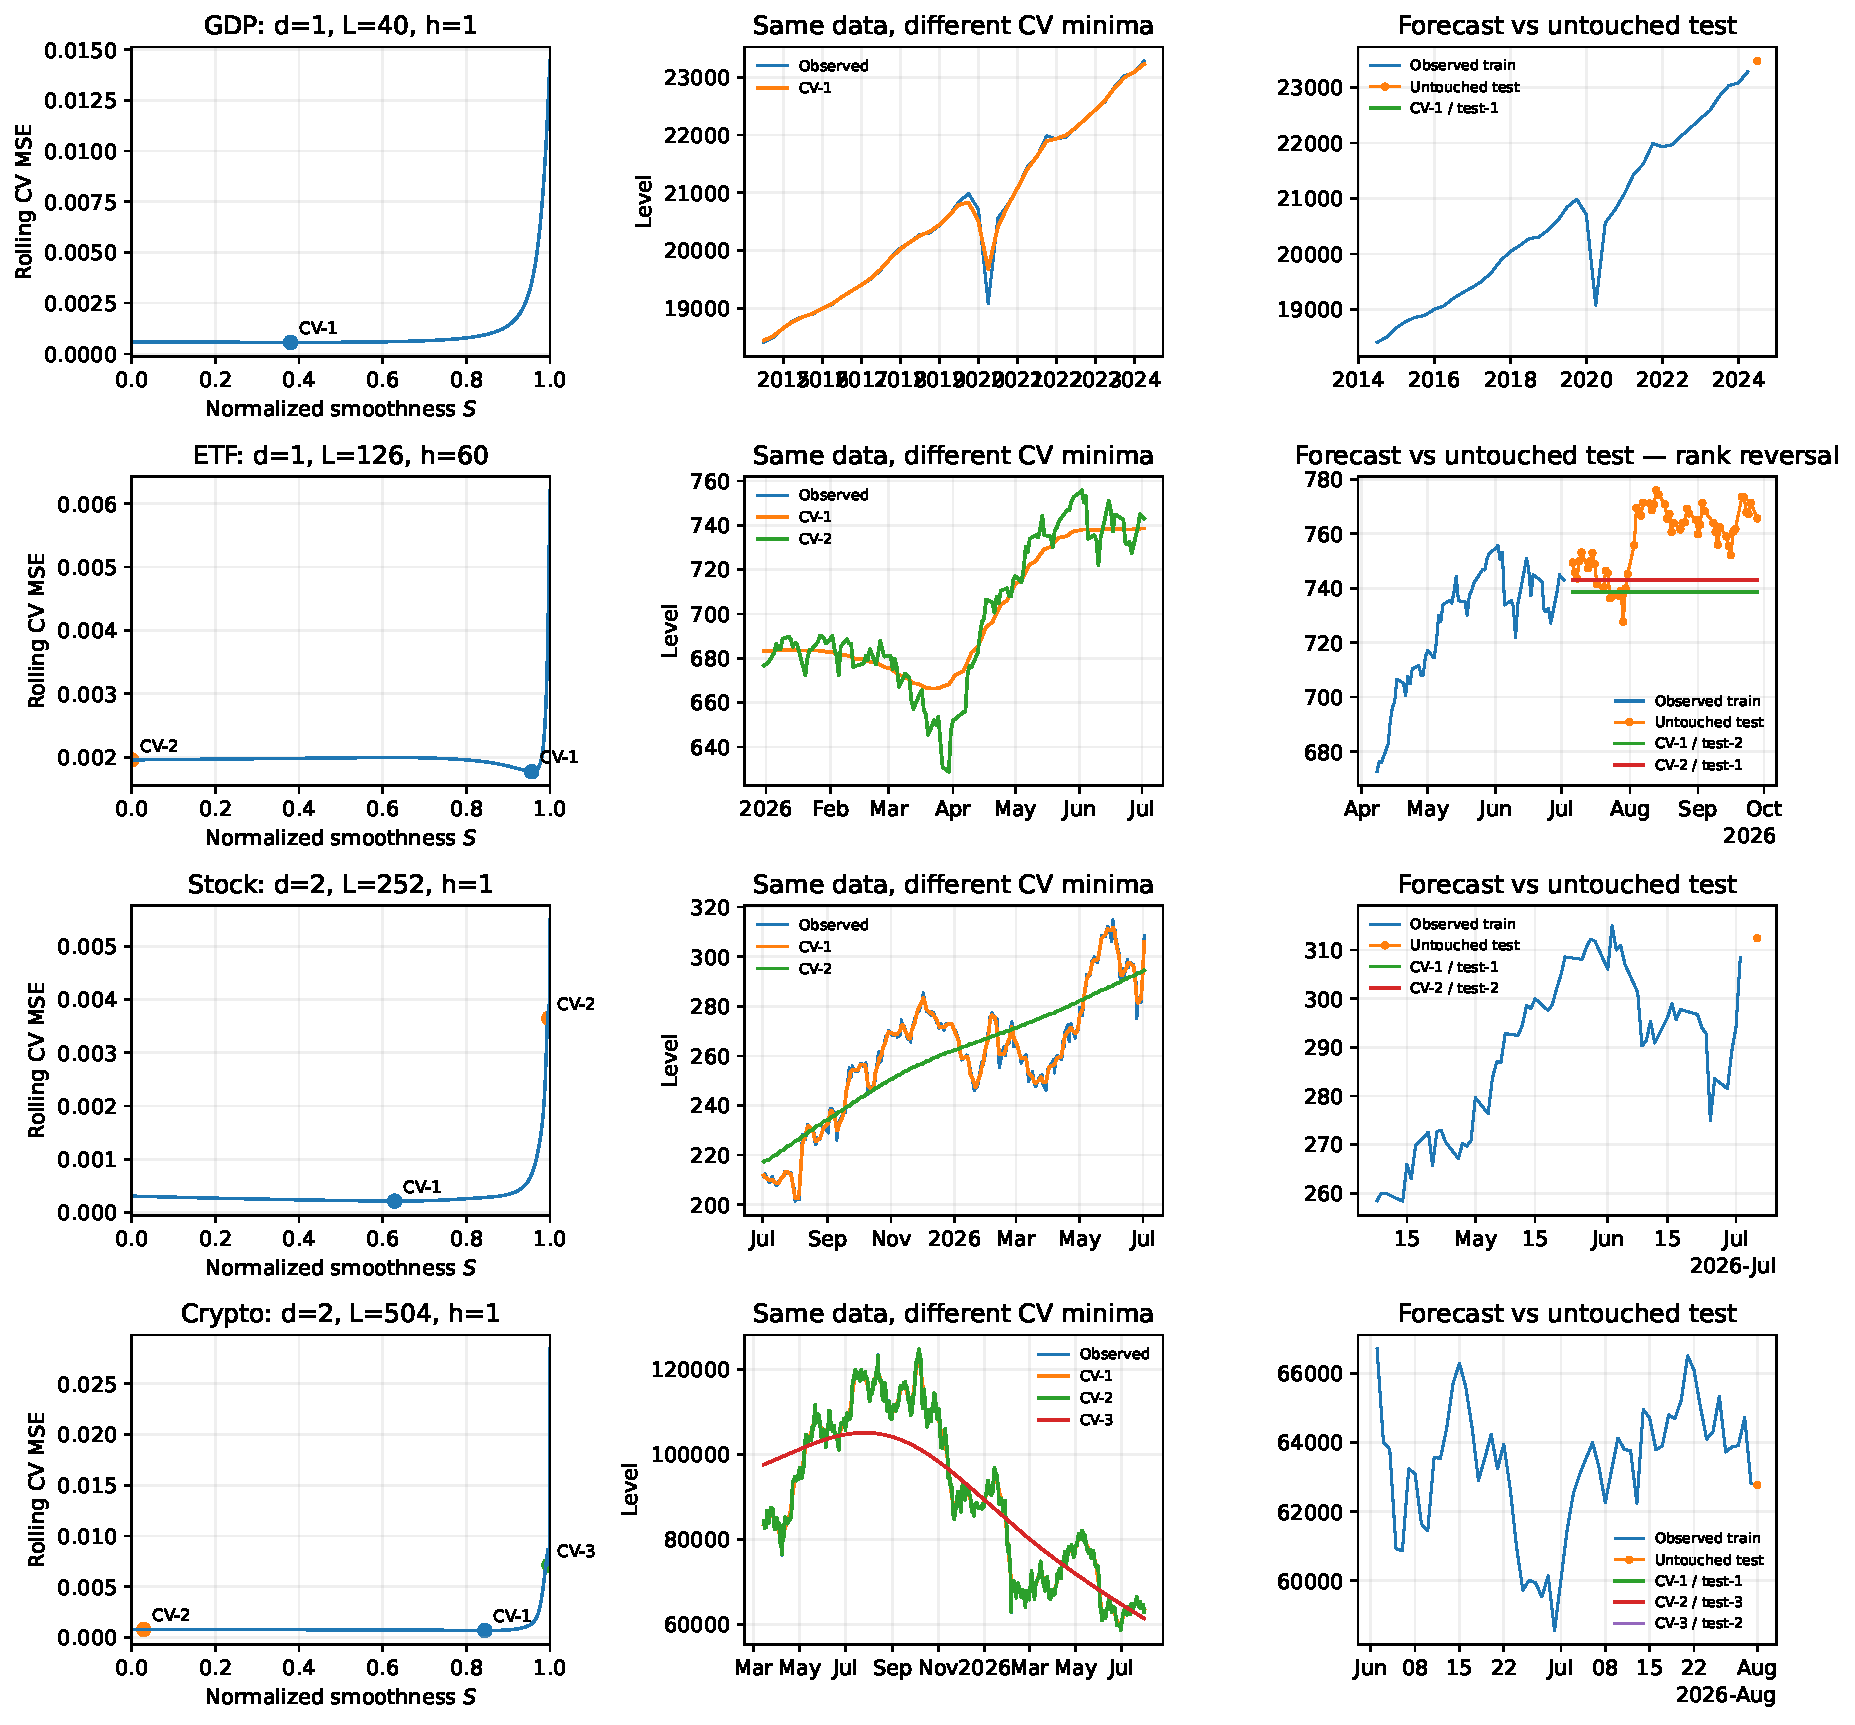
\includegraphics[width=\textwidth]{../results/numerical_smoothness_selection/20261001T022610Z_applied-paper_72b8aaa/applied_case_studies.pdf}
\caption{Applied interpretation of forecast-CV minima. Each row corresponds to
GDP, SPY, AAPL, or BTC--USD. The left panels show the development-region
forecast-CV profile and representative minima; the center panels show trend
estimates fitted to the same final development window; the right panels compare
the frozen candidate forecasts with the untouched test block. Candidate labels
retain validation rank even when the later test ranking differs.}
\label{fig:applied}
\end{figure}

The test comparison is not used to replace rolling CV by retrospective test
selection. Its role is to reveal selection sensitivity: when several local
minima exist, the validation winner need not dominate every later realization.
Recovering the candidate set therefore provides information that a single
unimodal optimization run would discard.



\subsection{Worked exact Sturm example}
\label{sec:sturm_example}

To illustrate the algebraic root count independently of the
large-window performance study, consider the exact rational
data
\begin{equation}
\label{eq:sturm_example_data}
L=6,\quad d=2,\quad h=2,\qquad
x=(4,0,-2,-1,3,1)^\top,\quad z=(0,1)^\top.
\end{equation}
The native linear continuation produces a rational forecast-MSE
objective. Its derivative has a numerator polynomial of degree
ten and exactly three distinct positive real roots according
to the Sturm variation difference. The corresponding
approximate coordinates are
\begin{equation}
\label{eq:sturm_example_roots}
\begin{aligned}
(\lambda_1,S_1)&\simeq(0.146706,\;0.380475),\\
(\lambda_2,S_2)&\simeq(1.101543,\;0.718759),\\
(\lambda_3,S_3)&\simeq(31.808860,\;0.976961).
\end{aligned}
\end{equation}
The first and third points are local minima; the middle
point is a local maximum. The corresponding future-block
MSE values are approximately $0.594777$, $4.364744$,
and $0.264095$. The exact limiting endpoint losses are
\begin{equation}
\label{eq:sturm_example_endpoints}
F(0)=\frac{17}{2},\qquad
F(1)=\frac{169}{441}.
\end{equation}
Consequently the smallest candidate value in this
example is the interior minimum near $S_3=0.976961$,
not either endpoint. The exact Sturm count certifies
\emph{completeness of the positive stationary-root set}
for this rational example. The decimal root locations,
the reported smoothness coordinates, and the objective
values are numerical approximations; they are not
claimed to be rational isolating intervals themselves.
This example illustrates algebraic certification and
multimodality, but does not establish a computational
advantage of symbolic Sturm isolation for realistic
window lengths. The independent frozen adaptive-search
benchmarks above remain the evidence on large-window
efficiency.

\subsection{Observed branch persistence and correspondence limits}
\label{sec:tracking_results}

The existing four-series tracking run records 1392 initialized
branch--origin states across 16 series--order configurations. Of these,
924 were successfully matched to a new local minimum and 468 were
recorded as missing under the fixed temporal radius. These are
\emph{tracking-state counts}, not ground-truth success and failure rates:
a missing state may reflect disappearance of a minimum, movement beyond
the continuation radius, or an assignment decision. The count also
depends on the number of branches initialized at the first origin.
Consequently, the empirical continuation fraction does not estimate
the probability of preserving a physically meaningful branch label.

Figure~\ref{fig:tracked_examples} illustrates the tracked locations
under different difference orders in GDP, SPY, AAPL, and BTC--USD,
alongside Validation-2 forecast errors and an untouched test block.
This visualization shows that the matched paths can be used to build
chronological branch histories. The Val2 and final forecast panels
belong to the downstream decision layer; they are included only to
document what information the numerical correspondence interface
makes available.

\begin{figure}[p]
\centering
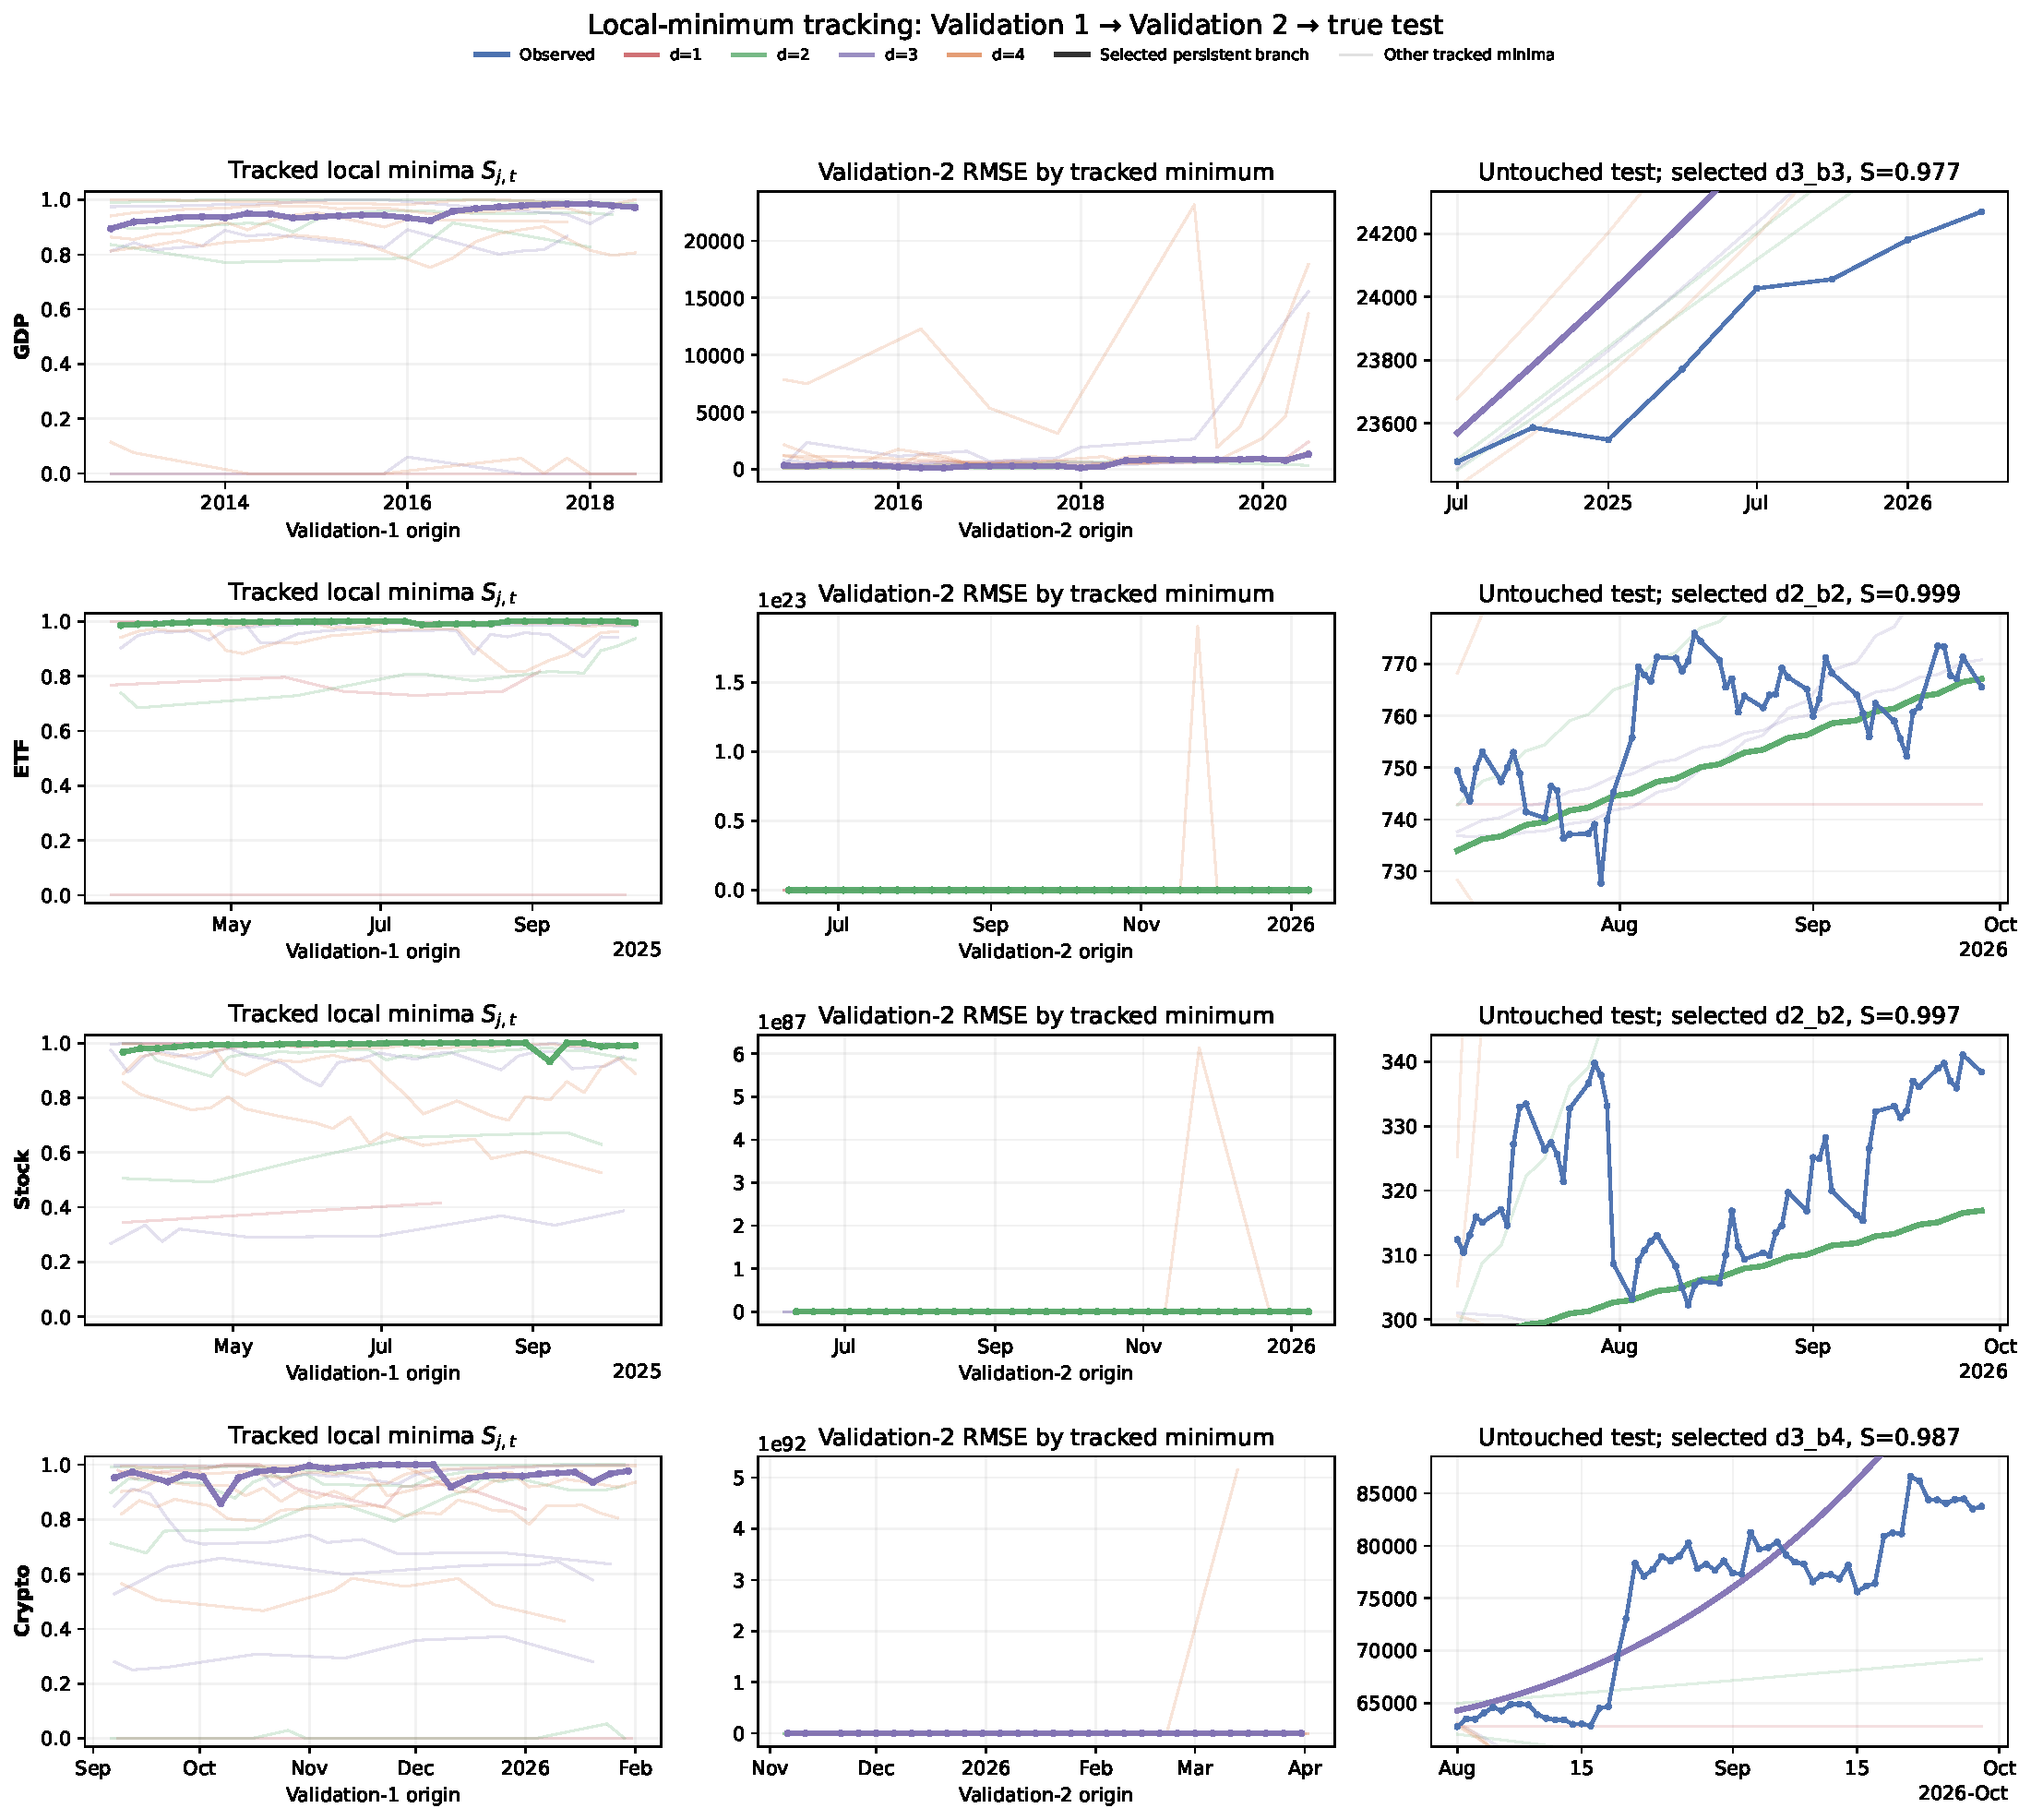
\includegraphics[width=\textwidth]{../results/numerical_smoothness_selection/20261002T074706Z_tracked-minima-paper_8fe5437/tracked_minima_validation.pdf}
\caption{An existing four-series temporal-minimum demonstration.
Left: tracked smoothness locations by difference order. Middle:
historical Validation-2 losses. Right: candidate forecasts on the
reserved test block. Highlighted branches were selected using
historical forecast information rather than an identity oracle. This figure demonstrates the interface and
does not validate numerical matching against known branch labels.}
\label{fig:tracked_examples}
\end{figure}

The explicit counterexample in Section~\ref{sec:tracking}
establishes that the greedy continuation algorithm can lose an
admissible branch match even when a globally maximum-cardinality
pairwise assignment would preserve both. Whether this happens
frequently on realistic paths, and how a pairwise-optimal assignment
behaves at genuine crossings, are empirical questions of the
controlled benchmark. Those results are not inferred from the
other forecast-error comparisons lacking known branch identities.

\section{Discussion}

The numerical benefit of the normalized smoothness coordinate is not that it makes the forecast objective convex. It does not. Its value is that it turns an unbounded penalty parameter into a compact, interpretable domain whose endpoints correspond to exact limiting estimators. Because \(S'(\lambda)>0\), stationary points and their local minimum/maximum classification are preserved in the interior. This allows the search to operate in a meaningful smoothness coordinate while derivative calculations continue to exploit the simple matrix dependence on \(\lambda\).

Compactification also creates a numerical issue: a large range of \(\lambda\) is compressed near \(S=1\). The early diagnostic runs showed that several derivative roots can occupy the same coarse upper-tail cell. Endpoint-aware refinement was introduced in response to that observed geometry, then frozen before the paper-scale benchmark. The subsequent sensitivity experiment independently reproduces the failure when endpoint refinement is removed. This is a useful example of a transformation that improves global search organization while still requiring explicit attention to its boundary geometry.

The paper's scope is narrower than general smoothing-parameter selection. The $S$ coordinate is the statistical and numerical reporting domain; auxiliary rational polynomial calculations in $\lambda$ are a way to certify roots, not a replacement for bounded smoothness selection. CV, GCV, information criteria, marginal likelihood, controlled smoothness, and simulation-calibrated HP parameters remain legitimate answers to their respective statistical objectives \cite{craven1979gcv,guerrero2008smoothness,cortes2017smoothness,biessy2026wh,franke2026hp}. Here the target is specifically rolling future-block forecast MSE. The contribution is therefore the numerical treatment of that criterion when multiple local minima are possible, together with the numerical correspondence problem that arises when those minima are followed across successive forecast origins. It is not a claim that forecast loss is universally preferable to the alternatives. The applied cases also show why retaining several detected minima can be informative: they form a finite set of distinct smoothing choices whose validation ranking may or may not persist out of sample. This candidate set should be interpreted as a selection-sensitivity diagnostic, not as a confidence set or probability distribution over smoothness.

Several limitations remain. The per-surface recovery experiments do not test
temporal label correctness, and the current greedy correspondence algorithm
is not globally pairwise optimal. Branches can approach or cross, new minima
may appear after initialization, and the tracking radius can be sensitive
to scale and step length. The controlled matching benchmark is therefore
needed before stronger temporal correspondence claims can be made.
First, no finite adaptive sampler can guarantee detection of every stationary root of an arbitrary smooth function without additional assumptions. Exact Sturm isolation provides a distinct, conditional guarantee only when the stationary equation is explicitly available as a manageable polynomial over the rationals. The adversarial stationary inflection illustrates this distinction: it is stationary but not a local minimum. Second, the dense reference grid is a benchmark rather than mathematical ground truth. Third, the analytic derivative formulas rely on a fixed affine trend-continuation operator. If additional forecasting parameters were re-estimated as functions of \(S\), for example inside an ARIMA continuation model, the derivative expressions would change. Finally, the financial experiment is only a real-data numerical stress test and provides no evidence of trading value or financial predictability.

The implementation, frozen experiment scripts, tracked data snapshots, and result summaries are available in the project repository at \url{https://github.com/heri-espino/Trend-Estimation}. The final benchmark inputs are versioned so the figures and tables in this paper can be regenerated from fixed result directories.

\section{Conclusions}

Forecast-optimal smoothness selection for penalized trend estimation can require more than minimizing a unimodal scalar function. By normalizing the controlled-smoothness coordinate to \(S\in[0,1]\), differentiating the chronological forecast-validation objective analytically, and searching adaptively for multiple local minima while retaining exact boundary candidates, the proposed procedure avoids an exhaustive dense scan of the smoothing domain.

Under a protocol frozen before the confirmatory experiments, the method recovered all relevant adversarial optima, all 2105 dense-reference minima across 1920 synthetic forecast surfaces, and all 473 dense-reference minima across 384 financial real-data surfaces. The synthetic and financial benchmarks required on average only 1.57\% and 1.84\% of the corresponding dense-grid evaluation counts. Sensitivity analysis identified endpoint refinement as the principal structural safeguard near the compactified upper boundary. In the applied case studies, separated minima occurred for several SPY, AAPL, and BTC--USD configurations but not for GDP, and one frozen SPY candidate set exhibited a validation--test rank reversal.

These results support the adaptive per-surface search as an accurate and computationally economical numerical procedure for the tested rolling forecast-validation problems. They do not establish universal recovery of all stationary points. The additional Sturm method gives a rigorous root count and isolating intervals for exact rational small-window objectives; it has not been benchmarked on the large-window datasets and cannot be substituted into the frozen cost comparisons. Correspondence of recovered minima across adjacent surfaces is a second numerical problem studied here, independent of the stationary-root search. That tracking layer is conceptually separate from root recovery: the observed 924 matches among 1392 recorded branch--origin states establish only that the existing method can produce usable branch histories. They do not establish correct cross-time identity. A simple two-branch counterexample shows that greedy continuation can lose an admissible link, and a controlled pairwise-assignment benchmark is the necessary next validation step. The overall method is intended as numerical support for forecast-based PLS smoothness selection rather than as a replacement for other statistical smoothing criteria.

\bibliographystyle{abbrv}
\bibliography{bibliografia}

\end{document}
